\chapter{Introduction}
Since ever, earthquakes have been a threat to human settlements and for centuries, scientists dedicated their work to describe them. It is only after Alfred Wegener postulated the drift of tectonic plates in 19.. [cite...] that a comprehensive model is available. The earth crust is compound of several rigid plates driven by earth mantle convection and the friction between them is at the origin of earthquakes. The scientific understanding of the period preceding the rupture process, or nucleation, is still at its beginning, but is essential to predict earthquakes with enough lead time to evacuate populations. Geodesic monitoring of faults to associate unusual movements with imminent earthquakes [cite...] or small-scale experimental setups for the material weakening and rupture of rocks [cite...] have been conducted, but a lot more research has to be done. \\
Numerical simulations have proven to be useful tools, 

\chapter{Background and Theory}
\section{Simulating Sequences of Earthquake and Aseismic Slip (SEAS)}
\subsection{General SEAS model}
\label{ssec:GeneralSeasModel}
The SEAS model consists of two adjacent tectonic plates which move in opposite directions. The contact surface is called $fault$ and because of friction forces there, the plates progressively deform over years in the \textit{aseismic phase} until the internal force cause an abrupt relaxation within seconds, the \textit{earthquake}. Each plate is a linear elastic body, governed by the general equation of motion \ref{eq:GeneralEquationOfMotion}, directly derived from Newton's second law \cite{LinearElasticityTheory}.
\begin{equation}
	\label{eq:GeneralEquationOfMotion}
	\nabla \cdot \mathbf{\sigma} + F = \rho \pdv[2]{u}{t}
\end{equation}
In this equation, $\mathbf{\sigma}$ is the Cauchy stress tensor, $F$ are some external forces, $\rho$ is the density of the medium and $u$ the displacement vector at each point in the plate. This hyperbolic PDE solves any elastodynamic problem in an anisotropic nonhomogeneous material without yielding, where the components of stress and strain are linearly dependent. Hooke's law in \autoref{eq:HookesLaw} describes how the Cauchy stress tensor $\mathbf{\sigma}$ is calculated from the strain $\mathbf{\varepsilon}$, which itself comes from the gradient of the displacement. The Einstein summation notation is used throughout the thesis and all indices stand for the three space dimensions.
\begin{equation}
\label{eq:HookesLaw}
\mathbf{\sigma}_{ij} = \mathbf{C}_{ijkl}\mathbf{\varepsilon}_{kl} = \frac{1}{2}\mathbf{C}_{ijkl}\left(\pdv{u_k}{x_l} + \pdv{u_l}{x_k}\right)
\end{equation}
The stiffness tensor $\mathbf{C}$ describes all material properties and because of symmetry requirements only contains 21 different entries. The stress tensor $\mathbf{\sigma}$ has components $\sigma_i$ for the normal stress, linked to a compression or dilatation, and for the shear stress $\tau_{ij}$, which changes the shape of the body. 
\begin{equation}
\label{eq:CauchyStressTensor}
\mathbf{\sigma} = \begin{pmatrix}
\sigma_1 & \tau_{12} & \tau_{13} \\ \tau_{21} & \sigma_2 & \tau_{23} \\ \tau_{31} & \tau_{32} & \sigma_3
\end{pmatrix}
\end{equation}
In the aseismic phase, the displacement evolves uniformly, such that the second time derivative of the displacement can be assumed to be zero, such that the problem is simplified to the elliptic PDE of elastostatics in \autoref{eq:GeneralElastostaticProblem}.
\begin{equation}
\label{eq:GeneralElastostaticProblem}
\nabla \cdot \mathbf{\sigma} + F = 0
\end{equation}
It means that we consider the plate to be in an elastostatic equilibrium at any moment of time. This assumption does not hold for the earthquake which is characterized by sudden changes in the displacement, and especially the so devastating shock waves that propagate from the epicenter cannot be represented. However, in this thesis, the main focus is on predicting when an earthquake is triggered in the aseismic phase, and this loose assumption is kept for the earthquake, such that one model is sufficient to simulate the whole range of SEAS. \\

In the seismic model from \cite{MechanicsOfEarthquakeRupture}, the fault is split in two sections: below a depth of approximately $24$km, the two tectonic plates slip smoothly skid past each other at a constant slip rate $V_p$. The upper section of the fault comes along with a friction law, In \autoref{chap:2DSEAS}, a simplified model in two dimensions is described, in which only slip and shear tress orthogonal to the domain is considered. 

\begin{figure}[H]
	\centering
	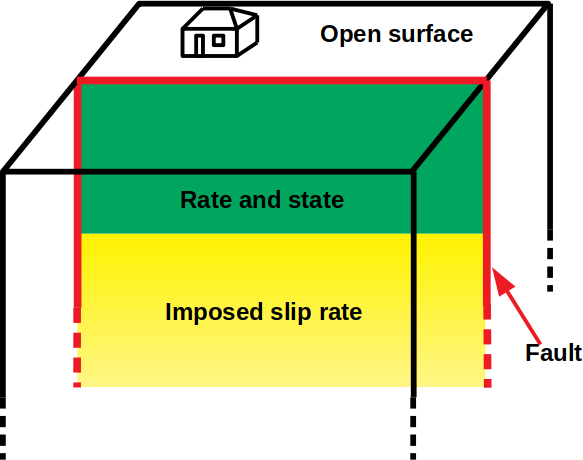
\includegraphics[width=0.3\textwidth]{images/generalSEASModel.png}
	\label{fig:general3DSEASModel}
	\caption{General setup of the SEAS model. Up to a depth $W=24$km, the slip is calculated with rate-and-state friction and everywhere below, the slip is driven by an imposed slip rate}
\end{figure}

To quantify the shift that builds up over time, the slip $S$ is introduced to measure the distance between the displacements $u^+$ and $u^-$ on the two plates that shared a common initial point on the fault. The normal vector $n$ of the fault surface points from "+" to "-". As a direct consequence of the slip, the slip rate $V$ describes the relative velocity between the plates.
\begin{align}
	\label{eq:DefinitionSlipAndSlipRate}
	S &= \left(\mathbf{I}-nn^T\right)\left(u^- - u^+\right) \\
	V &= \frac{dS}{dt}
\end{align}
At the fault, the normal stress $\sigma_n = n_i\mathbf{\sigma}_{ij}n_j$ induces, together with some friction coefficient $f$, the fault strength $\tau_S$. In general, a friction law defines a force in opposite direction to the velocity, and in this particular case, the force magnitude is $\tau_S$. To preserve the force equilibrium along the fault, the internal shear stress $\tau_i=(\delta_{ij}-n_in_j)\mathbf{\sigma}_{jk}n_k$ has to cancel out this traction term from the fault. 
\begin{align}
	\tau_S &= \sigma_n f \\
	\tau &= \tau_S\frac{V}{\norm{V}} 
\end{align}
As pointed out by \cite{GeneralSEASSimulations}, the quasi-static model described in \autoref{eq:GeneralElastostaticProblem} cannot handle this velocity-dependent shear traction and needs an additional damping term. For this purpose, we introduce the factor $\eta=\rho c_S/2$ which depends on the density $\rho$ and on the shear wave speed $c_S$. Both parameters are characteristic to the medium and do therefore not change over time. This leads to \autoref{eq:GeneralFrictionLaw}, which will be called \textit{friction law} throughout the thesis. 
\begin{align}
	\label{eq:GeneralFrictionLaw}
	0 &= \norm{\tau} - \sigma_n f - \eta \norm{V}
\end{align}

\subsection{Friction at the fault}
\label{ssec:FrictionLaws}
To calculate the coefficient $f$, an appropriate friction law is required. A common framework is the rate and state friction law, which contains a state variable $\theta$ to describe the ageing of the fault. Dieterich \cite{Dieterich79}\cite{Dieterich81} and Ruina \cite{Ruina} developed an empirical model in \autoref{eq:GeneralFrictionCoefficient} to define the friction in function of the slip rate $V$ and the state variable $\theta$. 
\begin{align}
	\label{eq:GeneralFrictionCoefficient}
	f(V,\theta) &= f_0 + a\ln(\frac{V}{V_0}) + \theta
\end{align}
The constant parameters $f_0$ and $V_0$ stand for the steady-state sliding, that is, if the slip rate reaches $V=V_0$, the state variable vanishes and and the friction is equal to $f_0$. In the SEAS model, the parameters $f_0$ and $\theta$ are summed up to form a new state variable $\psi = f_0 +\theta$, which takes the value of $f_0$ at steady-state sliding. With the summation rule for logarithms, the two terms can be combined in a single logarithm $a\ln(\frac{V}{V_0}e^{\frac{\psi}{a}})$. For very small values of $V$, the logarithm might fail, and a standard remedy \cite{Lapusta} is to replace it by the inverse hyperbolic sine function. 
\begin{align}
\label{eq:SEASFrictionCoefficient}
	f(V, \psi) &= a\cdot \text{arsinh}\left(\frac{V}{2V_0}e^{\frac{\psi}{a}}\right)
\end{align}

The state variable $\theta$ is a measure for the maturity of contacts, such that the older a fault gets, the stronger it is. A slip over a distance $L$ is sufficient to renew the contact and reset the state variable to 0. This motivates the definition of the ageing law $g^*(\theta, V) = \frac{b}{L}\left(V - V_0e^{\frac{\theta}{b}}\right)$ to describe the change rate of the state variable. For $\psi$, the ageing law reads: 

\begin{align}
	\label{eq:GeneralAgeingLaw}
	\frac{d\psi}{dt} = g(\psi, V) &= \frac{bV_0}{L}\left(e^{\frac{f_0 - \psi}{b}} - \frac{V}{V_0}\right)
\end{align}

The parameters $a$ and $b$ describe the material strength under velocity weakening and strengthening and are defined empirically from the experiment in \autoref{fig:DependencyParametersAandB}. The value for $b=0.015$ is chosen constant, and $a$ takes the value $a_0=0.010$ until a depth $h=3$km, it then increases linearly until $a_{max}=0.025$ at a depth $H=15$km, where it remains for greater depths. 

\begin{figure}[H]
	\centering
	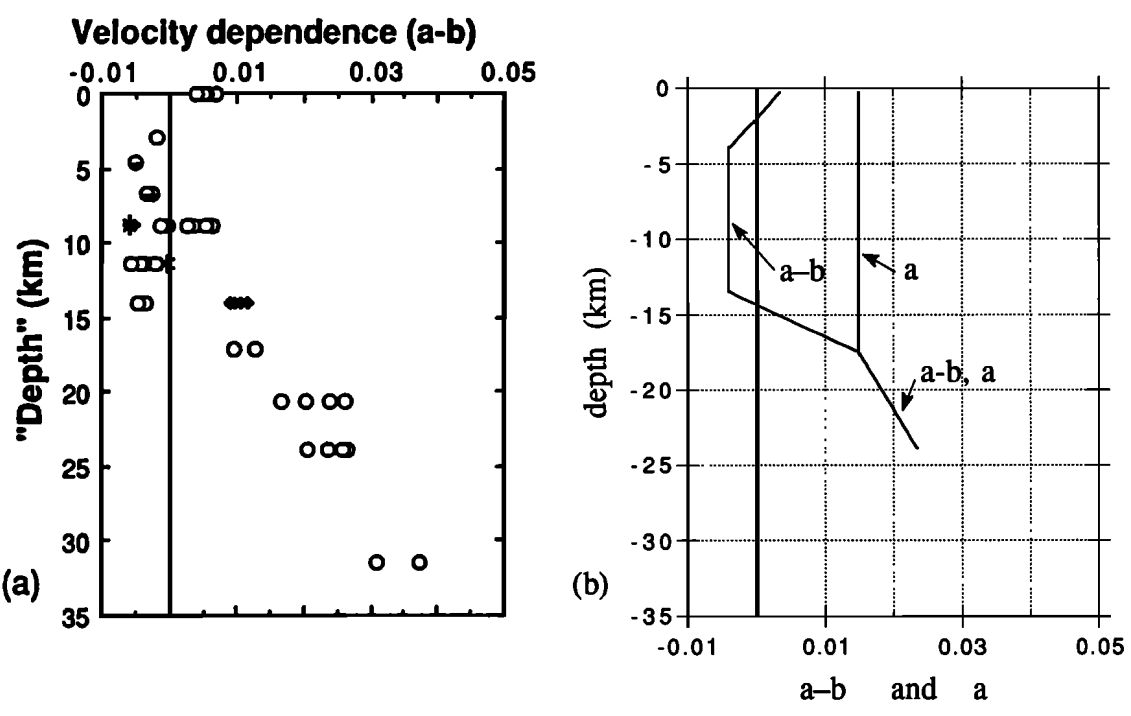
\includegraphics[width=0.7\textwidth]{images/ParametersAandBExperimental.png}
	\label{fig:DependencyParametersAandB}
	\caption{Experimental data for granite under hydrothermal conditions on velocity weakening/strengthening in (a) and simplified model for $a$ and $b$ as used in SEAS in (b). Figure taken from \cite{GeneralSEASSimulations}}
\end{figure}




\section{Differential Algebraic Equations (DAE)}

All in all, the SEAS time problem can be resumed to a first order differential algebraic equation (DAE):
\begin{align}
	\label{eq:GeneralSEASDAE}
	\begin{cases}
		\frac{dS}{dt} = V  & \text{(slip rate)} \\
		\frac{d\psi}{dt} = g(\psi, V) = \frac{bV_0}{L}\left(e^{\frac{f_0 - \psi}{b}} - \frac{V}{V_0}\right) & \text{(ageing law)} \\
		\;\,\ 0 = f(S,\psi,V) = \tau(S) - a \sigma_n(S) \text{arsinh}\left(\frac{V}{2V_0}e^{\frac{\psi}{a}}\right)\frac{V}{\norm{V}} - \eta V & \text{(friction law)}
	\end{cases}	
\end{align}
In general, DAEs differ from ODEs by the fact that the right-hand side of time derivatives cannot be calculated directly and require to solve an algebraic first. In our case, the slip rate $V$ is needed to evaluate the terms $\frac{dS}{dt}$ and $\frac{dV}{dt}$ but is not available from the solution vector. Instead, the algebraic equation of the friction law needs to be solved for $V$ first, and because of its complexity, it requires an iterative nonlinear solver. For this problem, there exist essentially two approaches: either $V$ is iteratively calculated at each evaluation of the right-hand side of the time derivatives or $V$ is added as an additional component to the solution vector when implicit time integration methods are used. Both approaches, [in addition to two others, buy the premium subscription to get access to all formulations], are investigated in detail in \autoref{chap:44rmulations4SEAS}. \\
From theory, the current problem is a semi-explicit DAE of index 1 \cite[p. 168]{DAETheory}, because the Jacobian $\pdv{f}{V}$ is not singular (a detailed analysis can be found in \autoref{sssec:Jacobian_ODE}). In general, it is very hard to prove the consistency and stability of a DAE


\section{Time-adaptive Time Integration Methods}
Earthquake simulations represent events that occur at several time scales. In the aseismic slip phase, timesteps of the order $h=10^7s$ are sufficient whereas during the earthquake, the rapid changes require timestep sizes as little as $h=10^{-3}s$. To adapt the timestep size from one step to the next, an estimate of the local truncation error is needed which indicates whether the stepsize should be increased or decreased. This section presents two families of time integrators, explicit Runge-Kutta and implicit BDF schemes, that come along with such an estimate.

\subsection{Explicit RK methods}
The Runge-Kutta methods are a class of one step method, which calculate the solutions at $s$ intermediate stages to obtain the next timestep. We will only consider the explicit, time-adaptive RK methods. For a general ODE $\dot{x} = f(t,x)$ and a stepsize $h$, The next solution $x_{n+1}$ is calculated from the current solution $x_n$ as: 
\begin{equation}
	x_{n+1}	= x_n + h\sum_{i=1}^{s}b_ik_i
\end{equation}
The terms $k_i$ stand for the evaluation of the right-hand side at the different stages and are calculated iteratively as:
\begin{align}
	k_i = f\left(t_n + c_ih, x_n + h\sum_{j=1}^{i-1}a_{ij}k_j\right)
\end{align}
For adaptive time-stepping, an estimate of the local truncation error is needed in addition. It is obtained by: 
\begin{equation}
	\varepsilon	= h\sum_{i=1}^{s}(b_i - \bar{b}_i)k_i
\end{equation}
The coefficients $\bar{b}_i$ usually stand for another RK scheme with either higher or lower order. All coefficients are commonly represented in a Butcher tableau, sketched below.
\begin{center}
\begin{tabular}{c | c c c c c }
	$0$ & & & & & \\
	$c_2$ & $a_{21}$ & & & & \\
	$c_3$ & $a_{31}$ & $a_{32}$ & & & \\  
	$\vdots$ & & & $\ddots$ & & \\
	$c_s$ & $a_{s1}$ & $a_{s2}$ & $\cdots$ & $a_{s,s-1}$ & \\ \hline
	& $b_1$ & $b_2$ & $\cdots$ & $b_{s-1}$ & $b_s$ \\ 
	& $\bar{b}_1$ & $\bar{b}_2$ & $\cdots$ & $\bar{b}_{s-1}$ & $\bar{b}_s$ 
\end{tabular}
\end{center}

An overview of the Butcher tableaus used in this thesis can be found in \autoref{apx:ButcherTableaus}.

\subsection{Implicit BDF methods}
Implicit methods are well-suited to solve stiff problems and allow for higher timesteps than explicit methods. Instead of evaluating the time-derivative in the right-hand side of an ODE for a known slution $\psi_n$, it is evaluated at the next timestep with $\psi_{n+1}$, which is not known. This requires solving an algebraic equation at each timestep without an analytic expression at hand for it. BDF (Backward Differentiation Formula) methods offer a convenient framework for implicit methods up to the order $p=6$. They are multi-step methods, where a method of order $p$ requires the solutions at the $p$ previous timesteps.  \\
A general description of the time-adaptive BDF coefficients can be obtained with the derivatives of the Lagrange interpolation polynomial. If one has a BDF method of order $k$, the coefficients $\alpha_{n+i}$ in front of the previous $k$ solutions are needed to calculate the new solution $\psi_{n+k}$.
\begin{equation}
	\sum_{i=0}^{k}\alpha_{n+i}\psi_{n+i} = f(\psi_{n+k},V_{n+k}) \approx \dot{\psi}_{n+k}
\end{equation} 

To approximate the time derivative $\dot{\psi}_{n+k}$ at the new solution, one could find the polynomial $L(t)$ that interpolates all points $(t_{n+i}, \psi_{n+i})$ and calculate its derivative at the last point $t_{n+k}$. This polynomial $L(t)$ is exactly the Lagrangian interpolation polynomial, calculated as:
\begin{equation}
	L(t) = \sum_{i=0}^{k}\psi_{n+i}\ell_i(t) \qquad\text{with}\qquad \ell_i(t) = \prod_{\substack{0\le j\le k \\j \ne i}}\frac{t-t_{n+j}}{t_{n+i}-t_{n+j}}
\end{equation}

We want to express the derivative $\dot{L}(t)$ at the specific time $t=t_{n+k}$, so that we can approximate $\dot{\psi}_{n+k} \approx \dot{L}(t_{n+k})$ For that, we first need the derivatives of the Lagrange basis polynomials $\dot{\ell}_i(t)$. Because of $\dot{L}(t_{n+k}) = \sum_{i=0}^{k}\dot{\ell}_i(t_{n+k})\psi_{n+k}$, it can be seen that if we evaluate $\dot{\ell}_i(t)$ at the time $t=t_{n+k}$, we obtain exactly the wanted coefficients $\alpha_{n+i}$. The basis polynomials can be calculated with the product rule:
\begin{equation}
	\alpha_{n+i} := \dot{\ell}_i(t_{n+k}) = \sum_{\substack{0\le m\le k \\m \ne i}}\left[\frac{1}{t_{n+i}-t_{n+m}}\prod_{\substack{0\le j\le k \\j \ne i,m}}\frac{t_{n+k}-t_{n+j}}{t_{n+i}-t_{n+j}}\right]
\end{equation}
Alternatively, the time-adaptive BDF coefficients can be derived from Taylor expansions, as described in \autoref{apx:BDF_derivation_Taylor} for the first three schemes.

\subsubsection{Error estimate with a higher-order BDF scheme}
\label{sssec:errorEstimateBDFEmbeddedScheme}
To evaluate the local truncation error at a given timestep, a similar approach as for the time-adaptive Runge-Kutta can be used. If a scheme of order $k$ is used, it involves solving the system a second time with order $k+1$. The error estimate is then the norm of the difference between the two calculated solutions. An obvious drawback of this method are the high computational costs, since the evaluation of the error estimate is as expensive as calculating the solution at the next timestep and requires to calculate the right-hand side of the ODE several times, which might be an expensive operation. Another limitation of this method is that the 6th order BDF scheme cannot be used for the time integration, since it implies to calculate a 7th order solution for the error estimate, which is not possible because the BDF method is only stable up to the order $k=6$. 

\subsubsection{Error estimate with Lagrange polynomials}
\label{sssec:errorEstimateBDFLagrange}
With the derivatives of the Lagrangian polynomial, a new possibility to estimate the error appears. Once the solution $\psi_{n+k}$ is found, the derivative $\dot{\psi}_{n+k}$ is first approximated with the last $k$ solutions, which gives the coefficients $\alpha_i$, and then with the last $k+1$ solutions, which results in the set of coefficients $\beta_i$. Now, assume that the $k$th-order approximate results in a perturbed $\dot{\psi}'_{n+k}$ and the $(k+1)$th-order approximates the exact $\dot{\psi}_{n+k}$. We have:
\begin{equation}
	\sum_{i=0}^{k}\alpha_{n+i}\psi_{n+i} = \dot{\psi}'_{n+k} \qquad \text{and}\qquad \sum_{i=-1}^{k}\beta_{n+i}\psi_{n+i} = \dot{\psi}_{n+k} \\
\end{equation}
We now want to find the perturbation $\epsilon$ in $\psi_{n+k}$ which is the reason for the different approximations $\dot{\psi}_{n+k}$ and $\dot{\psi}'_{n+k}$. We set:
\begin{align}
	\sum_{i=0}^{k-1}\alpha_{n+i}\psi_{n+i} + \alpha_{n+k}(\psi_{n+k} + \epsilon) &= \sum_{i=-1}^{k}\beta_{n+i}\psi_{n+i} \\
	\Leftrightarrow
	\epsilon &= \frac{1}{\alpha_{n+k}}\left(\beta_{n-1}\psi_{n-1} + \sum_{i=0}^{k}(\beta_{n+i}-\alpha_{n+i})\psi_{n+i}\right)
\end{align}
This expression for $\epsilon$ can be used as an estimate for the local truncation error instead of calculating the difference to a higher order BDF method. The main advantage is that the nonlinear system does not need to be solved twice in one timestep.

\subsubsection{Adaptive BDF order}
\label{sssec:adaptiveBDFOrder}
Which one of the six BDF methods is best appropriate to solve the problem is not an easy task to determine in ahead, as the ideal order of the scheme might change throughout the simulation. Generally speaking, a high order gives the best results when the timestep size remains approximately constant between the timestes, whereas low orders are more appropriate if the timestep size currently increases or decreases a lot. The idea is to find at the end of a timestep an optimal BDF order for the next step. \\
If $k_n$ denotes the current order of the scheme, one can evaluate the error estimate if a scheme of order $k_n-1$, $k_n$ or $k_n+1$ was used. We then obtain three values for the error estimate $\epsilon_-$, $\epsilon$ and $\epsilon_+$. This is easy to calculate with the Lagrangian polynomials, since it only requires to calculate the coefficients $\alpha_i$ for the considered order and sum up the weighted solution vectors. For the embedded higher-order BDF scheme it is also possible, but requires then in total four executions of the Newton iteration in one step, which is very likely not worth it. \\
Next, one calculates the factors $f_-$, $f$ and $f_+$ to change the timestep size $h_n$ from the current step to the next step $h_{n+1} = fh_n$. For the most basic timestep adapters with a safety factor $C$, this gives: 
\begin{equation}
	f_- = C{\epsilon_-}^{-1/k_n} \qquad \text{,}\qquad 
	f   = C{\epsilon}^{-1/(k_n+1)} \qquad \text{and}\qquad 
	f_+ = C{\epsilon_+}^{-1/(k_n+2)}
\end{equation}
One then finds the largest of the three factors, and decreases the order by one if it is $f_-$, remains at the same order if it is $f$ and increases the order by one if it is $f_+$. Of course, one has to ensure that the new order $k_{n+1}$ remains in the range $[1,6]$. 

\section{A Different Approach: Physically Motivated Time-Stepping}
Lapusta et al \cite{Lapusta} proposed a strategy to select the evolution timestep $h_{ev}$ with respect to the current state of the field variables. It shall fulfill respond to two observations: first, slow particle velocities should allow for large timesteps, and second, the relative displacement in each timestep should be small compared to the characteristic slip evolution distance $L$. Together with the local slip rate $V_i$ and a cell parameter $\xi_i$, the evolution timestep can be defined as:
\begin{equation}
	h_{ev} = \min_i\left[\xi_i L_i / V_i \right]
\end{equation}
The parameter $\xi_i$ depends on the time integration method, the space discretization of the domain, the environment slip rate and the stress gradient and is essentially chosen such that a perturbation at a single node always dies away. Additionally, $\xi_i$ has to be smaller than $1/2$, to avoid that within a timestep, a cell is displaced by more than half the characteristic slip distance $L_i$. \\
This approach is probably fruitful and should always be kept in mind, however this thesis does not investigate it further. Instead, timesteps are only defined through the error estimates of the numerical schemes. Moreover, the divergence issues addressed to define the parameter $\xi_i$ only apply to explicit time integrators with restricted numerical stability and do not pose any problems for implicit methods, whose convergence conditions are much less restrictive.